\section{Sharpness: the extremal systems}\label{sec:extremal}

\subsection{The square root $R$}

Let $R$ be the branch of $\sqrt{(z^2-a^2)(z^2-b^2)}$ that is analytic in
$\C\setminus S$ and satisfies $R(z)=z^2\big(1+O(z^{-2})\big)$ at infinity. It
exists because a loop around one component of $S$ encircles two branch
points.\footnote{Each of the four factors $(z\mp a)^{1/2}$, $(z\mp b)^{1/2}$ changes sign along a loop around its branch point; a loop around $[a,b]$ changes the sign twice, so the product returns to its value.}

\begin{lemma}\label{lem:R}
$R(-z)=R(z)$ and $R(\bar z)=\overline{R(z)}$. On the real axis,
$R(t)=\sqrt{(t^2-a^2)(t^2-b^2)}>0$ for $\abs t>b$,
$R(t)=-\sqrt{(a^2-t^2)(b^2-t^2)}<0$ for $\abs t<a$, and
\[
R(t+i0)=i\,r(t),\quad R(-t+i0)=-i\,r(t)\qquad(a<t<b).
\]
\end{lemma}

\begin{proof}
The symmetries hold because $R(-z)$ and $\overline{R(\bar z)}$ are branches of
the same root with the same behaviour at infinity. Near $z=b$,
$R(z)=(z-b)^{1/2}G(z)$ with $G$ analytic and $G(b)=\sqrt{2b(b^2-a^2)}>0$, the
root being positive for $z>b$. Passing from $t>b$ to $t<b$ through $\Cp$ turns
$(z-b)^{1/2}$ into $i\sqrt{b-t}$, so $R=ir$ on $(a,b)$. Near $z=a$ write
$R=(z-a)^{1/2}G_1(z)$ with $(z-a)^{1/2}>0$ for $t>a$; then $G_1$ is
positive imaginary on $(a,b)$, and passing to $t<a$ through $\Cp$ gives
$R=i\sqrt{a-t}\,G_1<0$. The values on the negative axis follow from the
symmetries.
\end{proof}

\subsection{The extremal system for constant phase}

Put
\begin{equation}\label{eq:m-tau}
m^2=b^2\,\frac{E(k)}{K(k)},\qquad
\tau_\star=\frac{2\theta K(k)}{\pi b}=\frac{4\theta K(\kappa)}{\pi(a+b)} ,
\end{equation}
so that $a^2<m^2<b^2$, because $m^2=I_2/I_0$ is an average of $t^2$ over
$(a,b)$ (\cref{prop:J}), and define
\begin{equation}\label{eq:hstar}
h_\star(z)=\tau_\star\int_0^z\frac{s^2-m^2}{R(s)}\dd s,\qquad H_\star=e^{ih_\star}.
\end{equation}

\begin{theorem}\label{thm:extremal}
Let $\theta>0$.
\begin{enumerate}
\item[(i)] The integral \eqref{eq:hstar} does not depend on the path in
$\C\setminus S$; $h_\star$ is analytic there, odd, real on $\R\setminus S$,
and $h_\star(z)=\tau_\star z+O(z^{-1})$ at infinity.
\item[(ii)] On the band, $h_\star(x+i0)=\theta+i\alpha_\star(x)$ with
\begin{equation}\label{eq:alphastar}
\alpha_\star(x)=\tau_\star\int_a^x\frac{m^2-s^2}{r(s)}\dd s ,
\end{equation}
which is positive on $(a,b)$, vanishes at $a$ and $b$, and is largest at
$x=m$.
\item[(iii)] $h_\star$ is a Herglotz function, and $H_\star$ is a zero-free
passive system, regular on the band, lossless on $\R\setminus S$, with
constant phase $\theta$ on $[a,b]$ and
\[
\frac1{b-a}\int_a^b\alpha_\star(\omega)\dd\omega=\theta\Lambda .
\]
\end{enumerate}
\end{theorem}

\begin{proof}
(i) The integrand is even, analytic in $\C\setminus S$, and integrable at the
four branch points. A loop around $[a,b]$ can be shrunk onto the two sides of
the cut, where $R=\pm ir$; its integral is $\pm2i\int_a^b(s^2-m^2)\dd s/r(s)
=\pm2i(I_2-m^2I_0)=0$. By evenness the same holds around $[-b,-a]$. Hence
$h_\star$ is single-valued, and odd. On $(-a,a)$ and on $\abs t>b$ the
integrand is real, so $h_\star$ is real there; it is also real along the
path from $0$ to $\pm a$, and the vanishing of the periods shows that it
returns to real values beyond $\pm b$. At infinity,
$(s^2-m^2)/R(s)=1+O(s^{-2})$, so $h_\star(z)-\tau_\star z$ tends to a constant;
it is odd and analytic for $\abs z>b$, so its Laurent series has only odd
powers and the constant is $0$.
(ii) For $0<x<a$, $h_\star(x)=\tau_\star\int_0^x(m^2-s^2)\dd s/\sqrt{(a^2-s^2)(b^2-s^2)}$
by \cref{lem:R}, and at $x=a$ this is
\begin{align*}
&\tau_\star\Big(\frac{m^2}bK(k')-b\big(K(k')-E(k')\big)\Big)\\
&\quad=\frac{\tau_\star b}{K(k)}\big(E(k)K(k')+E(k')K(k)-K(k)K(k')\big)\\
&\quad=\frac{\pi b\,\tau_\star}{2K(k)}=\theta ,
\end{align*}
by the substitution $s=a\sin\phi$\footnote{It gives $\dd s/\sqrt{(a^2-s^2)(b^2-s^2)}=\dd\phi/(b\sqrt{1-k'^2\sin^2\phi})$, and $\int_0^{\pi/2}\sin^2\phi\,\dd\phi/\sqrt{1-k'^2\sin^2\phi}=(K(k')-E(k'))/k'^2$ with $a^2/k'^2=b^2$.} and Legendre's relation
(\cref{app:elliptic}). Continuing from $a$ along the upper side of the cut,
where $R=ir$,
\[
h_\star(x+i0)=\theta+\tau_\star\int_a^x\frac{s^2-m^2}{ir(s)}\dd s=\theta+i\alpha_\star(x).
\]
The integrand of \eqref{eq:alphastar} is positive for $s<m$ and negative for
$s>m$, and its integral over $(a,b)$ is $I_2-m^2I_0=0$; so $\alpha_\star$
rises from $0$ at $a$ to its maximum at $m$ and falls back to $0$ at $b$.
(iii) The function $v=\Im(h_\star-\tau_\star z)$ is harmonic in $\Cp$,
continuous on $\overline{\Cp}$, tends to $0$ at infinity by (i), vanishes on
$\R\setminus S$, and equals $\alpha_\star\ge0$ on $(a,b)$ and, by the symmetry
$h_\star(-\bar z)=-\overline{h_\star(z)}$, also on $(-b,-a)$. By the minimum
principle $v\ge0$, so $\Im h_\star\ge\tau_\star\Im z\ge0$. Thus $h_\star$ is a
Herglotz function with $h_\star(iy)\in i\R$, $H_\star$ is passive and zero-free,
and it is regular on the band since $h_\star$ is continuous up to $(0,\infty)$.
As $\Im h_\star=0$ on $\R\setminus S$, \eqref{eq:stieltjes} shows
$\mu_\star(\R\setminus S)=0$, and \cref{thm:main} holds with equality.
\end{proof}

\begin{remark}\label{rem:extremal}
The extremal system is a delay $\tau_\star$ at high frequency, as its
asymptotics shows, yet its group delay on the band is zero, its phase being
constant there. All of its attenuation is in the band, and none of its
response outside the band is reactive: in the language of
\eqref{eq:foster} it has $\beta=\tau_\star$ and a measure carried by $S$. For an
octave and $\theta=1$, $\tau_\star=0.6864/a$, $m=1.4988\,a$, and the peak
attenuation is $\alpha_\star(m)=0.3482$\,Np, against the mean $0.2735$.
\Cref{fig:extremal} shows $\alpha_\star$ for several band ratios, and
\cref{fig:hstar} the function $\Im h_\star$ over $\Cp$.
\end{remark}

\begin{figure}[t]
\centering
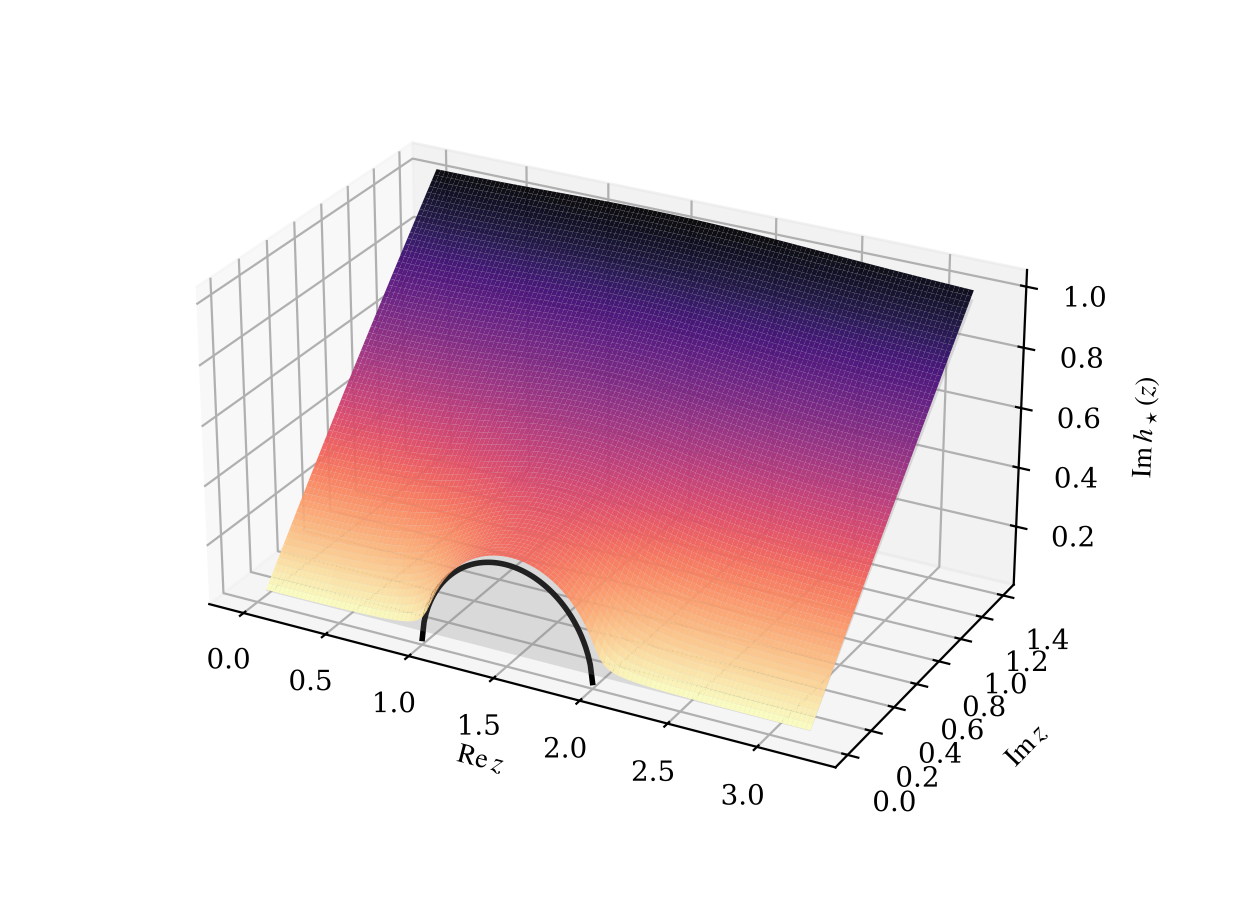
\includegraphics[width=\columnwidth]{figures/fig_hstar.png}
\caption{The surface $\Im h_\star(x+iy)$ over the upper half-plane for an
octave and $\theta=1$. It is positive in $\Cp$, as a Herglotz function must
be; on the real axis it vanishes off the band, and over the band its
boundary values are the attenuation $\alpha_\star$ (black curve). Far from
the band it approaches the plane $\tau_\star y$ (grey) of the delay.}
\label{fig:hstar}
\end{figure}

\begin{figure}[t]
\centering
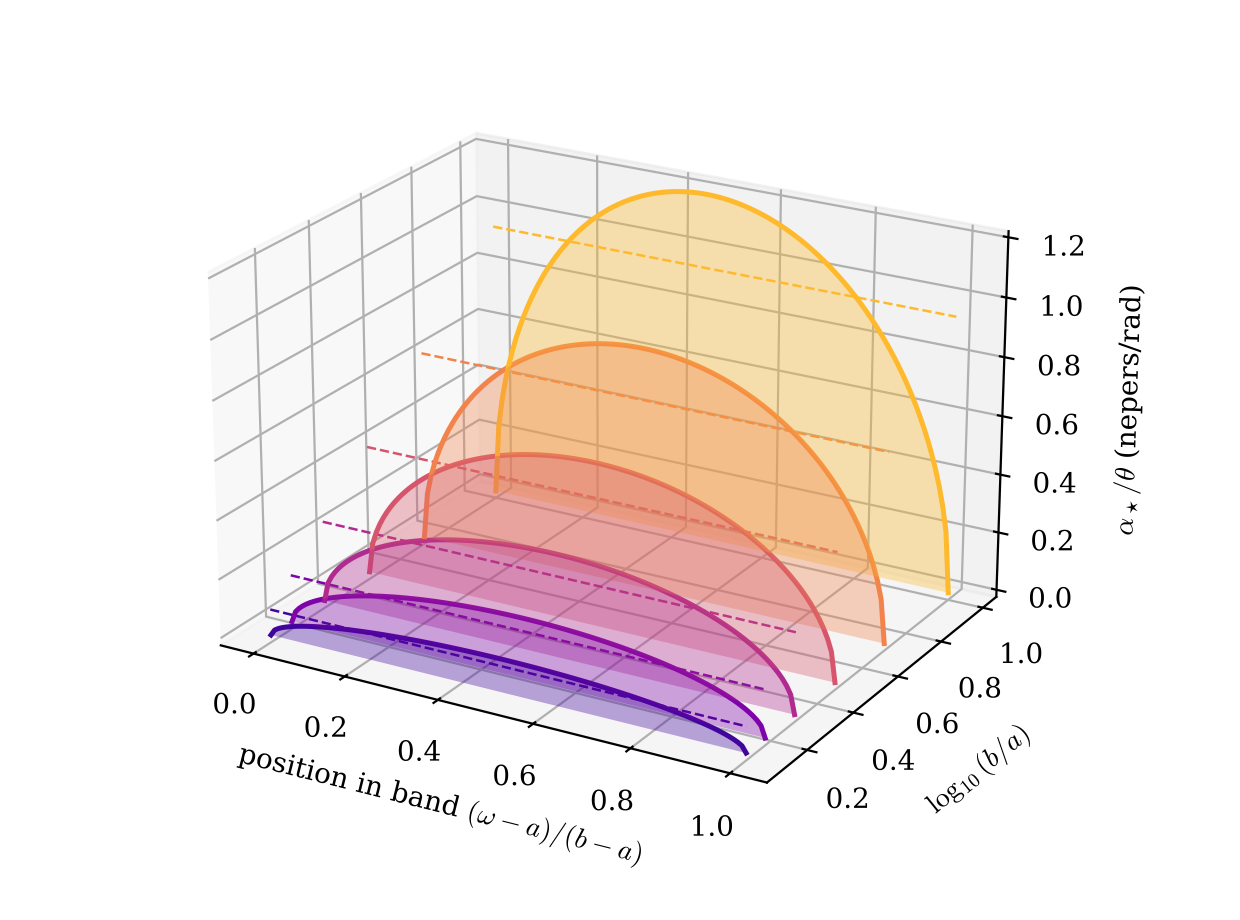
\includegraphics[width=\columnwidth]{figures/fig_extremal.png}
\caption{The attenuation $\alpha_\star/\theta$ of the extremal system across
the band, for $b/a=1.25,1.5,2,3,5,10$. Dashed lines mark the mean,
$\Lambda$. The profile vanishes at both edges.}
\label{fig:extremal}
\end{figure}

\subsection{Extremal systems for other phases}

The construction extends to phases that are not constant, and this is what
we need for systems with zeros.

\begin{proposition}\label{prop:profile}
Let $g$ be continuously differentiable on $[a,b]$ and put
\begin{gather*}
h_g(z)=\frac{2zR(z)}\pi\int_a^b\frac{g(t)}{r(t)\,(z^2-t^2)}\dd t,\\
\beta_g=\frac2\pi\int_a^b\frac{g(t)}{r(t)}\dd t .
\end{gather*}
\begin{enumerate}
\item[(i)] $h_g$ is analytic in $\C\setminus S$, odd, real on
$\R\setminus S$, continuous up to $S$ from both sides, and
$h_g(z)=\beta_gz+O(z^{-1})$ at infinity.
\item[(ii)] For $a<x<b$, $\Re h_g(x+i0)=g(x)$ and
\[
\Im h_g(x+i0)=v_g(x)=\frac{2x\,r(x)}\pi\PV\int_a^b\frac{g(t)}{r(t)\,(x^2-t^2)}\dd t .
\]
\item[(iii)] If $v_g\ge0$ on $(a,b)$ and $\beta_g\ge0$, then $e^{ih_g}$ is a
zero-free passive system, regular on the band, with phase $g$ and
attenuation $v_g$ on the band and no measure outside $S$, so that
$\int_a^bv_g=\frac12\int_a^bg\,p$.
\item[(iv)] For constant $g=\theta$, $h_g=h_\star$.
\end{enumerate}
\end{proposition}

\begin{proof}
(i) The Cauchy integral $q(z)=\int_a^bg(t)\,(r(t)(z^2-t^2))^{-1}\dd t$ is
analytic off $S$ and even; $zR(z)q(z)$ is odd and real on $\R\setminus S$
because $R$ is real there (\cref{lem:R}). The density $g/r$ has
singularities of order $\abs{t-a}^{-1/2}$, $\abs{t-b}^{-1/2}$ at the ends, so
$q$ is $O(\abs{z-a}^{-1/2})$, $O(\abs{z-b}^{-1/2})$ there and H\"older
continuous up to the open cut \cite[Ch.~4]{muskhelishvili}; multiplied by
$R$, which vanishes like the square root, the product is continuous up to
$S$. At infinity $q(z)=z^{-2}\int_a^bg/r+O(z^{-4})$ and
$zR(z)=z^3(1+O(z^{-2}))$, which gives the expansion.
(ii) Write $2z/(z^2-t^2)=1/(z-t)+1/(z+t)$. By the Plemelj formula, at
$x+i0$ with $a<x<b$ the first part of $q$ contributes
$\PV\int g\,(r(t)(x-t))^{-1}\dd t-i\pi g(x)/r(x)$, so
\[
\frac2\pi xq(x+i0)=\frac{2x}\pi\PV\int_a^b\frac{g(t)\dd t}{r(t)(x^2-t^2)}-\frac{ig(x)}{r(x)} .
\]
Multiplying by $R(x+i0)=ir(x)$ gives the real part $g(x)$ and the imaginary
part $v_g(x)$.
(iii) As in the proof of \cref{thm:extremal}(iii), $\Im(h_g-\beta_gz)$ is
harmonic, continuous up to the axis, zero on $\R\setminus S$, equal to
$v_g\ge0$ on $S$, and tends to $0$ at infinity; so $\Im h_g\ge\beta_g\Im
z\ge0$. The last identity is \cref{thm:sumrule}.
(iv) Let $d=h_g-h_\star$. Both functions have real part $\theta$ on the upper
side of $(a,b)$, are real on $\R\setminus S$ and satisfy $h(\bar
z)=\overline{h(z)}$, so on the lower side the real part is again $\theta$ and
$d(x\pm i0)=\pm i\,e(x)$ with $e$ real and continuous. Since $R(x\pm i0)=\pm
ir(x)$, the function $d/R$ has the same boundary values $e/r$ from both
sides of $(a,b)$, and likewise on $(-b,-a)$. It is therefore analytic across
the open cuts, by Morera's theorem, and its singularities at $\pm a,\pm b$
are $O(\abs{z-c}^{-1/2})$, hence removable. So $d/R$ is entire. Both
functions have the linear term $\tau_\star z$, because
$\beta_\theta=2\theta I_0/\pi=\tau_\star$, so $d=O(z^{-1})$ and $d/R\to0$ at
infinity. Thus $d=0$.
\end{proof}

\begin{lemma}\label{lem:positivity}
If $g(t)/t$ is nonincreasing on $[a,b]$, then $v_g\ge0$. In particular
this holds when $g>0$ and $g$ is nonincreasing, and then also $\beta_g>0$.
\end{lemma}

\begin{proof}
Substitute $\sigma=t^2$ and write $G(\sigma)=g(\sqrt\sigma)/\sqrt\sigma$,
which is nonincreasing. Then
\[
\frac{g(t)\dd t}{r(t)}=\frac{G(\sigma)\dd\sigma}{2\sqrt{(\sigma-a^2)(b^2-\sigma)}},
\]
and with $\sigma_0=x^2$,
\begin{multline*}
v_g(x)=\frac{x\,r(x)}\pi\\
\times\PV\int_{a^2}^{b^2}\frac{G(\sigma)}{(\sigma_0-\sigma)
\sqrt{(\sigma-a^2)(b^2-\sigma)}}\dd\sigma .
\end{multline*}
Glauert's integral \cite{king},
\[
\PV\int_{A}^{B}\frac{\dd\sigma}{(\sigma_0-\sigma)\sqrt{(\sigma-A)(B-\sigma)}}=0
\]
for $A<\sigma_0<B$,
which follows from the substitution $\sigma=\frac{A+B}2-\frac{B-A}2\cos\phi$
and $\PV\int_0^\pi\dd\phi/(\cos\phi-\cos\phi_0)=0$, allows us to subtract
$G(\sigma_0)$:
\[
v_g(x)=\frac{x\,r(x)}\pi\int_{a^2}^{b^2}\frac{G(\sigma)-G(\sigma_0)}{\sigma_0-\sigma}
\frac{\dd\sigma}{\sqrt{(\sigma-a^2)(b^2-\sigma)}} .
\]
For a nonincreasing $G$ the difference quotient is nonnegative, so
$v_g\ge0$. If $g>0$ is nonincreasing, $g/t$ is decreasing, and $\beta_g>0$
is clear.
\end{proof}
